% !TeX root = ../apuntes-ea.tex

\chapter{Biyecciones}

\section{El por qué de la notación cíclica}

\begin{dfn}[Conjunto de biyecciones]
	Sea $X$ un conjunto. Definimos
	\begin{align*}
		\biy{X} = \{f: X \to X \mid f \text{ es biyección}\}
	\end{align*}
\end{dfn}

Como coinciden dominio y codominio ($f:X \to X$) si $f$ es inyectiva entonces automáticamente es sobre y por tanto biyectiva.

En general, tiene sentido pensar en $Biy(X)$ aunque $|X| = \infty$. Además, en dicho conjunto viven la biyección identidad y la biyección inversa para cada biyección. Por tanto, tiene sentido pensar en $(Biy(X), \circ)$ como un grupo (la composición de biyecciones da una biyección). Lo escribimos en forma de teorema.

\begin{thm}
	Sea $X$ un conjunto. El par $(\biy{X}, \circ)$ es un grupo.
\end{thm}

Nos concentraremos en el caso en el que $|X| = n < \infty$ que nos da $Biy(X) = S_n$. Ver \autoref{dfn:sn} para una explicación detallada del grupo $S_n$.

Fijamos un conjunto $X$ y un homomorfismo de grupos $\alpha: X \to Biy(X)$. A partir de estos datos definimos una relación de equivalencia que nos da una partición de $X$, es decir, vamos a partir $X$ en conjuntos disjuntos. Veamos un ejemplo particular.

\begin{ej}
	Supongamos $G = X,\ |G| = n$ y consideramos $\rho: G \to \autom{G} \subset Biy(X)$. Definimos la relación en $X = G$
	\begin{align*}
	aRb \iff \exists g \in G \mid \phi_g(a) = b,\ \phi_g(x) = gx\inv{g}
	\end{align*}
	que es la relación de conjugación dada por el isomorfismo de conjugación de toda la vida.
	
	Ahora, en lugar de pensar en $G = X$ pensamos en $X = \{H < G\}$ (los subgrupos de $G$). Para cualquier isomorfismo de grupos $\beta: G \to G$, tenemos que si $H < G$ entonces $\beta(H) < G$.
	
	Lo que hemos hecho aquí es un caso particular de lo que viene ahora.
\end{ej}

Ahora pasamos al caso general.

\begin{pro}
	Sea $\alpha: G \to Biy(X),\ g \mapsto \alpha(g)$ un homomorfismo de grupos\footnote{Ojo: aquí las imágenes de los elementos $g \in G$ son biyecciones $f:G \to G$, por eso tendrá sentido la notación $\alpha(g)(a)$ que significa aplicar la función que nos devuelve $\alpha$ al elemento $a \in G$.}. Definimos la relación de equivalencia $R$ en el conjunto $X$
	\begin{align}
	aRb \iff \exists g \in G \mid \alpha(g)(a) = b
	\end{align}
	Afirmamos que la relación es de equivalencia y que nos divide $X$ en subconjuntos disjuntos (nos particiona $X$).
\end{pro}

\begin{proof}Probamos las 3 propiedades de las relaciones de equivalencia.
	\begin{enumerate}
		\item Reflexiva: $\forall x \in X, a R a$. Por ser $\alpha$ homomorfismo tenemos que $\alpha(e_G) = id_X$ y por tanto $\alpha(e_G)(a) = a$.
		\item Simétrica: $aRb \implies bRa$. Partimos de que $\exists g \in G \mid \alpha(g)(a) = b$. Tomamos $\inv{g} \in G$ y por ser $\alpha$ homomorfismo de grupos tenemos que $\alpha(\inv{g})(b) = \inv{(\alpha(g))}(b) = a$.
		\item Transitiva: $aRb \land bRc \implies aRc$. Partimos de que $\exists g, g' \in G \mid \alpha(g)(a) = b \land \alpha(g')(b) = c$. Tomamos $g'g \in C$ y tenemos que $\alpha(g'g)(a) = \alpha(g')(\alpha(g)(a)) = \alpha(g')(b) = c$ por composición de biyecciones.
	\end{enumerate}
\end{proof}

¿Cómo son las clases que da la partición?

Pues tenemos que para $a \in X$, la clase $cl(a) = \{\alpha(g)(a) \mid g \in G\}$. Definimos $H_a = \{g \in G \mid \alpha(g)(a) = a\}$. Tenemos por lo visto anteriormente que $H_a < G \land |cl(a)| = [G:H_a]$. Entonces tenemos lo siguiente:
\begin{itemize}
	\item En el caso en que $X = G$, es decir, que el conjunto $X$ tiene dentro \textit{elementos} de $G$, tenemos que $H_a = C(a)$ donde $C(a)$ es el centralizador de $a$ (\autoref{dfn:centralizador}).
	\item En el caso en que $X = \{H < G\}$, es decir, que el conjunto $X$ tiene dentro \textit{subgrupos} de $G$, tenemos que $H_a = N(a)$ donde $N(a)$ es el normalizador de $a$ (\autoref{dfn:normalizador}).
\end{itemize}

Vista la definición abstracta, lo que nos interesa de esto es aplicarlo a los grupos $S_n$ de los que hablábamos antes. En particular, ahora daremos una definición formal de ciclo para la notación que introdujimos en la \autoref{sec:notacionciclica}.

\begin{wrapfigure}{l}{0.3\textwidth}
	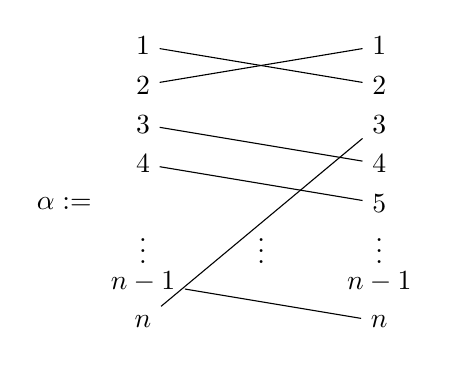
\begin{tikzpicture}
	\begin{scope}[scale=0.5]
	\node (alpha) at (-2, 0) {$\alpha :=$};
	\node (1) at (0,4) {$1$};
	\node (2) at (0,3) {$2$};
	\node (3) at (0,2) {$3$};
	\node (4) at (0,1) {$4$};
	\node (dots) at (0,-1) {$\vdots$};
	\node (nmenos1) at (0,-2) {$n-1$};
	\node (n) at (0,-3) {$n$};
	
	\node (1p) at (6,4) {$1$};
	\node (2p) at (6,3) {$2$};
	\node (3p) at (6,2) {$3$};
	\node (4p) at (6,1) {$4$};
	\node (5p) at (6,0) {$5$};
	\node (dotsp) at (6,-1) {$\vdots$};
	\node (nmenos1p) at (6,-2) {$n-1$};
	\node (np) at (6,-3) {$n$};
	
	\node (dotsc) at (3, -1) {$\vdots$};
	
	
	\draw (1) -- (2p);
	\draw (2) -- (1p);
	\draw (3) -- (4p);
	\draw (4) -- (5p);
	\draw (nmenos1) -- (np);
	\draw (n) -- (3p);
	\end{scope}
	\end{tikzpicture}
	\caption{La permutación $\alpha$ de $S_n$}
	\label{fig:permalphaejpart}
\end{wrapfigure}

Fijamos $\sigma \in S_n$ y definimos $G = \gen{\sigma}$ el subgrupo generado por $\sigma$ en $S_n$. Definimos ahora el homomorfismo
\begin{align*}
G = \gen{\sigma} & \to S_n = \biy{X},\qquad X = \{1, 2, 3, \dots, n\}
\end{align*}
Las clases $cl(i)$ para $i \in \{1, 2, \dots, n\}$ son de la forma\footnote{Las clases serían de la forma $\alpha(g)(i)$ pero es que en este caso todos los $\alpha(g)$ son elementos de $G = \gen{\sigma}$ y por tanto son de la forma $\sigma^k$.}
\begin{align*}
cl(i) = \{\sigma^k(i) \mid k \in \Z\}
\end{align*}


\begin{ej}
	Consideramos la permutación $\alpha \in S_n$ dada por (ver \autoref{fig:permalphaejpart})
	\begin{align*}
		\alpha = \begin{array}{ccccccc}
		1 & 2 & 3 & 4 & \dots & n-1 & n \\
		2 & 1 & 4 & 5 & \dots & n & 3
		\end{array}
	\end{align*}
	que en la notación cíclica podríamos escribir como $\alpha = (345\dots n)(12)$.
	
	En este caso la clase $cl(1) = \{1, 2\} = cl(2)$ está formada por los elementos que podemos obtener de aplicar $\alpha$ al elemento $1$. Ya se intuye la utilidad de la notación cíclica: la permutación $\alpha$ nunca mezcla elementos de la caja $\{1,2\}$ con elementos de la caja $\{3, 4, 5, \dots, n\}$. Así, también tendremos que $cl(3) = cl(4) = \dots = cl(n) = \{3, 4, 5, \dots, n\}$. Los elementos que hay en estas dos clases coinciden con los elementos que hay en cada uno de los ciclos en los que hemos descompuesto $\alpha$.
\end{ej}

Vemos que si fijamos $\sigma$ se define una partición en $\{1, \dots, n\}$ de subconjuntos disjuntos
\begin{align*}
F_1 \cup F_2 \cup \dots \cup F_n
\end{align*}

Si $r = |F_i| > 1$, $F_i = \{i_0, i_1, \dots, i_r\}$ tal que $\sigma(i_0) = i_1, \sigma(i_1) = i_2, \dots, \sigma(i_r) = i_0$.

\begin{dfn}[Ciclo]
	\label{dfn:ciclo}
	Diremos que $\sigma$ es un ciclo de longitud $r$ si en la partición definida
	\begin{align*}
	F_1 \cup F_2 \cup \dots \cup F_n
	\end{align*}
	todas las cajas $F_j,\ j < r$ tienen un único elemento y $F_r$ tiene $r$ elementos.
\end{dfn}

La definición quiere decir que, en el fondo, un ciclo es un tipo de permutación que al aplicarla sucesivamente sobre el conjunto $X$ lo particiona en varias cajas pero de manera que todas tienen un elemento excepto una, que tiene todos los elementos que se mueven entre ellos por la acción del ciclo. Un ejemplo en el conjunto $X = \{1, 2, 3, \dots, n\}$ sería

\begin{center}
	\begin{tabular}{|c|c|c|c|}
		\hline
		1 & 5 & \dots & \vdots \\\cline{2-4}
		2 & 6 & $\ddots$ & \vdots \\\cline{2-4}
		3 & $\ddots$ & $\ddots$ & \vdots  \\\cline{2-4}
		4 & \dots & \dots & n\\\hline
	\end{tabular}
\end{center}

Observemos que por la notación que hemos elegido, los ciclos tienen la estructura $(\sigma^0(a)\ \sigma^1(a)\ \sigma^2(a) \dots \sigma^s(a))$ donde $\sigma$ es un elemento de $S_n$ y $a$ un elemento de $X$. Dado que si $\sigma^k = Id$ entonces $\sigma^{k + i} = \sigma^i$, si \textit{rotamos} los números que definen el ciclo no estamos haciendo nada. Esto es, el ciclo $(1234) = (2341) = (3412) = (4123)$.

\section{De permutaciones a composiciones de ciclos}

\begin{pro}
	Toda biyección $\alpha \in S_n$ se puede expresar como composición de ciclos disjuntos dos a dos:
	\begin{align*}
		\alpha = \sigma_1 \circ \sigma_2 \circ \dots \circ \sigma_s
	\end{align*}
\end{pro}

\begin{pro}
	La composición de dos ciclos disjuntos conmuta, es decir, si $\sigma_1$ y $\sigma_2$ son ciclos disjuntos (que no comparten ningún elemento entre los paréntesis) entonces $\sigma_1 \circ \sigma_2 = \sigma_2 \circ \sigma_1$
\end{pro}

\begin{cor}
	Toda descomposición de una permutación $\alpha \in S_n$ en ciclos disjuntos $\alpha = \sigma_s \circ \sigma_{s-1} \circ \dots \circ \sigma_2 \circ \sigma_1$ se puede reordenar sin cambiar el resultado.
\end{cor}

\begin{ej}
	Antes de seguir veamos un ejemplo más de cómo una biyección de $S_n$ particiona el conjunto $X = \{1, 2, \dots, n\}$.
	
	Consideramos $\alpha \in S_n$ definida con
	\begin{align*}
		\alpha = \left(\begin{array}{cccccccccc}
		1 & 2 & 3 & 4 & 5 & 6 & 7 & 8 & 9 & 10 \\
		2 & 3 & 1 & 5 & 6 & 4 & 7 & 9 & 8 & 10
		\end{array}\right)
	\end{align*}
	
	La partición que nos da $\alpha$ de $X = \{1, 2, 3, 4, 5, 6, 7, 8, 9 10\}$ es la siguiente:
	\begin{center}
		\begin{tabular}{|c|c|c|c|}
			\hline
			1 & 4 & 7 & \\ \cline{3-3}
			2 & 5 & 8 & 10 \\
			3 & 6 & 9 & \\
			\hline
		\end{tabular}
	
		Partición de $X$ dada por $\alpha = (123)(456)(89)$
	\end{center}
	Esto lo obtenemos de buscar las clases de cada elemento. Empezamos por el que queramos, por ejemplo, el $1$:
	\begin{align*}
		cl(1) = \{\alpha^k(1) \mid k \in \Z\} = \{\alpha^0(1) = 1, \alpha^1(1) = 2, \alpha^2(1) = 3, \alpha^3(1) = 1, \alpha^4(1) = 2, \dots \}
	\end{align*}
	Eliminando duplicidades obtenemos que $cl(1) = \{1,2,3\}$. Análogamente obtenemos $cl(4) = \{4,5,6\},\ cl(7) = \{7\},\ cl(8) = \{8,9\},\ cl(10) = \{10\}$. Lo que hemos hecho es seguir el algoritmo descrito en la \autoref{sec:notacionciclica}, esta vez entendiendo el significado. Obtenemos que $\alpha = (123)(456)(89)$ o cualquier reordenación de los ciclos anteriores, ya que al ser disjuntos, cambiar el orden en el que los rotamos no afecta al resultado.
\end{ej}

\begin{wrapfigure}{l}{0.3\textwidth}
	\centering
	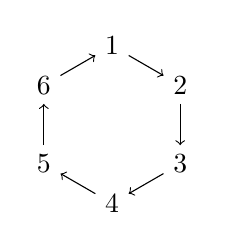
\begin{tikzpicture}
	\node (1) at (0,1) {${1}$};
	\node (2) at (0.866,0.5) {$2$};
	\node (3) at (0.866,-0.5) {$3$};
	\node (4) at (0, -1) {$4$};
	\node (5) at (-0.866, -0.5) {$5$};
	\node (6) at (-0.866,0.5) {$6$};
	
	\draw[->] 	(1) edge (2)
	(2) edge (3)
	(3) edge (4)
	(4) edge (5)
	(5) edge (6)
	(6) edge (1);
	\end{tikzpicture}
	\caption{El ciclo $\sigma = (123456)$}
	\label{fig:ciclo16}
	
	
	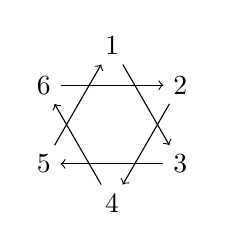
\begin{tikzpicture}
	\node (1) at (0,1) {${1}$};
	\node (2) at (0.866,0.5) {$2$};
	\node (3) at (0.866,-0.5) {$3$};
	\node (4) at (0, -1) {$4$};
	\node (5) at (-0.866, -0.5) {$5$};
	\node (6) at (-0.866,0.5) {$6$};
	
	\draw[->] 	(1) edge (3)
	(3) edge (5)
	(5) edge (1)
	(2) edge (4)
	(4) edge (6)
	(6) edge (2);
	\end{tikzpicture}
	\caption{El ciclo $\sigma^2 = (123456)^2$}
	\label{fig:ciclo16cuadrado}
	
	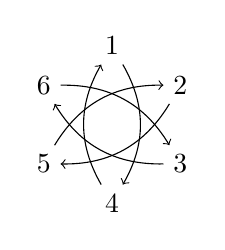
\begin{tikzpicture}
	\node (1) at (0,1) {${1}$};
	\node (2) at (0.866,0.5) {$2$};
	\node (3) at (0.866,-0.5) {$3$};
	\node (4) at (0, -1) {$4$};
	\node (5) at (-0.866, -0.5) {$5$};
	\node (6) at (-0.866,0.5) {$6$};
	
	\draw[->] 	(1) edge[bend left] (4)
	(4) edge[bend left] (1)
	(2) edge[bend left] (5)
	(5) edge[bend left] (2)
	(3) edge[bend left] (6)
	(6) edge[bend left] (3);
	\end{tikzpicture}
	\caption{El ciclo $\sigma^3 = (123456)^3$}
	\label{fig:ciclo16cubo}
\end{wrapfigure}

Veamos ahora cómo se relacionan los órdenes de los ciclos con su longitud.


\begin{ej}
	Consideramos $\sigma = (123456) \in \S_n$. Observamos que $\sigma^6 = Id$ es decir que $\sigma$ tiene orden 6.
	
	De esta manera si nos preguntan por $\sigma^{122} = (123456)^{122} = (123456)^{6\cdot20} \circ (123456)^2 = (123456)^2$ no nos asustamos.
	
	Si nos hubieran dado $\sigma$ con la notación habitual, aparte de que hubiera ocupado mucho, no podríamos haber resuelto esta operación tan rápido.
\end{ej}


\begin{ej}
	Nos preguntamos ahora por las potencias de $\sigma = (123456)$ menores que $6 = o(\sigma)$.
	\begin{itemize}
		\item $\sigma^2$ equivaldría a aplicar $\sigma$ dos veces a cada número $\{1, \dots, 6\}$ (los demás números no nos interesan porque sabemos que $\sigma$ no los mueve). Ayudándonos del dibujo obtenemos que $\sigma^2 = (135)(246)$.
		
		Se verifica que $\sigma^2$ tiene $o(\sigma^2) = 3$ y además si recordamos el \autoref{thm:ordendepotencia} comprobamos que se verifica $o(\sigma^2) = \frac{o(\sigma)}{mcd(o(\sigma), 2)} = \frac{6}{2} = 3$.
		
		\item En cuanto a $\sigma^3$ observamos que al aplicar $\sigma$ 3 veces nos quedan 3 ciclos y que se vuelve a verificar que $o(\sigma^3) =\frac{o(\sigma)}{mcd(o(\sigma), 3)} = \frac{6}{3} = 2$
	\end{itemize}
\end{ej}

Esto nos lleva a enunciar el siguiente teorema

\begin{thm}
	\label{thm:ordenpotenciasciclos}
	Sea $\sigma = (i_1\ i_2\ i_3 \dots i_n)$ un ciclo de longitud $n$. Sea $m \in \Z$ y $d = mcd(n,m)$. Entonces $\sigma^m$ es un producto de $d$ ciclos de longitud $\frac{n}{d}$ y estos son disjuntos dos a dos.
\end{thm}

Poder averiguar los órdenes de ciclos es una herramienta muy potente. Por ejemplo, podemos hacer lo siguiente.

\begin{ex}[H3.8]
	Demuestra que el subgrupo $G < S_4$ generado por los elementos $\sigma = (1432)$ y $\tau = (24)$ es isomorfo a $D_4$.
\end{ex}

\begin{proof}
	Sabemos que $o(\sigma) = 4$ y que $o(\tau) = 2$. Trabajando un poco vemos que
	\begin{align*}
		\gen{\sigma} &= \{\sigma = (1432), \sigma^2 = (13)(24), \sigma^3 = (4321), \sigma^4 = Id\} \\
		\gen{\tau} &= \{\tau = (24), \tau^2 = Id\}
	\end{align*}
	Faltaría ver que $\sigma \tau = \tau \sigma^3$ es decir que $(1432)(24) = (24)(4321)$ (spoiler: es verdad) y ya podríamos identificar $\sigma$ con $B$ y $\tau$ con $A$ para obtener la presentación del famoso grupo $D_4$:
	\begin{align*}
		D_4 \isom G = \gen{\sigma, \tau \mid o(\sigma) = 4 \land o(\tau) = 2 \land \sigma \tau = \tau \sigma^3}
	\end{align*}
\end{proof}

\begin{thm}
	Sea $\alpha$ una permutación expresada como composición de ciclos disjuntos $\alpha = \sigma_1 \circ \sigma_2 \circ \dots \circ \sigma_n$. Entonces el orden de $\alpha$ es el mínimo común múltiplo de los órdenes de cada $\sigma_i$:
	\begin{align*}
		\alpha = \sigma_1 \circ \sigma_2 \circ \dots \circ \sigma_n \text{ disjuntos } \implies o(\alpha) = mcm(\sigma_1, \dots, \sigma_n)
	\end{align*}
\end{thm}

% TODO demostrar esto: dorronsoro página 120

\begin{proof}
	Ver \cite[p.~120]{dor96}.
\end{proof}

\section{Sobre las conjugaciones de una descomposición en ciclos}

Antes de seguir, vamos a introducir dos proposiciones que nos serán de gran ayuda al calcular conjugados de una permutación, por ejemplo, para cuando queramos calcular centralizadores.

\begin{pro}
	Sea $\alpha \in S_n$ una permutación con descomposición en ciclos disjuntos
	\begin{align*}
	\alpha = \left(i_1^{(1)}\ i_2^{(1)}\ \dots\ i_{s_1}^{(1)}\right)\left(i_1^{(2)}\ i_2^{(2)}\ \dots\ i_{s_2}^{(2)}\right)\dots\left(i_1^{(r)}\ i_2^{(r)}\ \dots\ i_{s_r}^{(r)}\right)
	\end{align*}
	y sea $\omega \in S_n$. Entonces el conjugado de $\alpha$ por $\omega$ es $\alpha'$ y se obtiene de
	\begin{align*}
	\alpha' = \omega \alpha \inv{\omega} = \left(\omega(i_1^{(1)})\ \omega(i_2^{(1)})\ \dots\ \omega(i_{s_1}^{(1)})\right)\left(\omega(i_1^{(2)})\ \omega(i_2^{(2)})\ \dots\ \omega(i_{s_2}^{(2)})\right)\dots\left(\omega(i_1^{(r)})\ \omega(i_2^{(r)})\ \dots\ \omega(i_{s_r}^{(r)})\right)
	\end{align*}
\end{pro}

Se ve mejor con un ejemplo:

\begin{ej}
	Sea $\alpha = (123)(45) \in S_5$ y sea $\omega \in S_5$ alguna permutación. Entonces
	\begin{align*}
	\alpha' = \omega\alpha\inv{\omega} = \omega(123)(45)\inv{\omega}= \left(\omega(1)\ \omega(2)\ \omega(3)\right)\left(\omega(4) \omega(5)\right)
	\end{align*}
\end{ej}

También podemos ir en la otra dirección. Es decir, dados $\alpha$ y $\alpha'$ obtener $\omega$:

\begin{pro}
	Sean $\alpha, \alpha' \in S_n$ dos permutaciones cuyas descomposiciones en ciclos disjuntos son del mismo tipo y se denotan por
	\begin{align*}
	\alpha = \left(i_1^{(1)}\ i_2^{(1)}\ \dots\ i_{s_1}^{(1)}\right)\dots\left(i_1^{(r)}\ i_2^{(r)}\ \dots\ i_{s_r}^{(r)}\right) \\
	\alpha' = \left(j_1^{(1)}\ j_2^{(1)}\ \dots\ j_{s_1}^{(1)}\right)\dots\left(j_1^{(r)}\ j_2^{(r)}\ \dots\ j_{s_r}^{(r)}\right)
	\end{align*}
	Entonces $\exists \omega \in S_n$ tal que $\alpha' = \omega \alpha \inv{\omega}$ y $\omega$ se puede construir (en notación no cíclica)
	\begin{align*}
	\omega = \left(\begin{array}{ccccccccc}
	i_1^{(1)}\ &i_2^{(1)}\ &\dots\ &i_{s_1}^{(1)}\ & \dots\ &i_1^{(r)}\ &i_2^{(r)}\ &\dots\ &i_{s_r}^{(r)} \\
	j_1^{(1)}\ &j_2^{(1)}\ &\dots\ &j_{s_1}^{(1)}\ & \dots\ &j_1^{(r)}\ &j_2^{(r)}\ &\dots\ &j_{s_r}^{(r)}
	\end{array}\right)
	\end{align*}
\end{pro}

\begin{ej}
	Sean $\sigma, \sigma' \in S_5$. Busco $\tau \in S_5$ tal que $\sigma'$ sea conjugada de $\sigma$ por $\tau$, es decir, $\tau \in S_n \mid \sigma' = \tau\sigma\inv{\tau}$. Pues utilizamos el método
	\begin{align*}
	\begin{cases}
	\sigma 	&= (123)(45) \\
	\sigma' &= (245)(13)
	\end{cases} \longrightarrow \omega = \left(\begin{array}{ccccc}
	1 & 2 & 3 & 4 & 5 \\
	2 & 4 & 5 & 1 & 3
	\end{array}\right)
	\end{align*}
	o en notación cíclcia: $\omega = (124)(35)$.
\end{ej}

\section{Trasposiciones}

\begin{dfn}[Trasposición]
	Una trasposición es un ciclo de orden 2. Cualquier trasposición tiene orden 2.
\end{dfn}

Las trasposiciones tienen la forma $(a\ b)$ pero observemos que también se pueden escribir como $(b\ a)$ ya que lo que estamos haciendo es \textit{rotar} (o empezar en otro lugar del ciclo).

\begin{pro}
	La inversa de cualquier trasposición es ella misma.
\end{pro}

\begin{thm}
	El grupo $S_n$ está generado por las transposiciones $\sigma \in S_n$.
\end{thm}

Ya sabemos que cualquier permutación se puede expresar como producto de ciclos [disjuntos]. Para probar este teorema probaremos la siguiente proposición:

\begin{pro}
	Cualquier ciclo se puede expresar como composición de trasposiciones.
\end{pro}

La prueba es constructiva y describe la manera de expresar un ciclo como composición de trasposiciones.

\begin{proof}
	Sabemos que un ciclo $\sigma$ se escribe como $\sigma = (\sigma^0(a) = a\ \sigma^1(a)\ \sigma^2(a)\ \dots \ \sigma^s(a))$. Pues vasta con observar que la composición
	\begin{align*}
		\sigma = (a\ \sigma^s(a))(a\ \sigma^{s-1}(a))\dots(a\ \sigma^2(a))(a\ \sigma(a))
	\end{align*}
	tiene el mismo efecto.
\end{proof}

\begin{ej}
	La permutación $\sigma = (1234)$ se puede expresar como $\sigma = (14)(13)(12)$.
\end{ej}

\subsection{Paridad de las trasposiciones}

\begin{thm}
	\label{thm:paridadpermutaciones}
	Si $\sigma \in S_n$ se puede descomponer como un número par de trasposiciones entonces toda expresión en $\sigma$ expresada como una composición de un número par de trasposiciones.
	
	Análogamente para las permutaciones que se pueden expresar como una composición de un número impar de trasposiciones.
\end{thm}

\begin{proof}
	Definimos una función
	\begin{align*}
		S_n &\to GL_n(\N)\\
		\sigma &\mapsto \left(\begin{array}{ccc}
		e_\sigma(1) & \dots & e_\sigma(n) \\
		\vdots & \vdots & \vdots
		\end{array}\right)
	\end{align*}
	Esta función es un homomorfismo de grupos.
	
	Entonces si expresamos $\sigma$ como composición de trasposiciones $\sigma = (i_1^{(1)}\ i_2^{(1)})(i_1^{(2)}\ i_2^{(2)}) \dots (i_1^{(r)}\ i_2^{(r)})$ y aplicamos la función que hemos definido nos queda
	\begin{align*}
		A = \left(\begin{array}{ccc}
		e_\sigma(1) & \dots & e_\sigma(n) \\
		\vdots & \vdots & \vdots
		\end{array}\right) = \underbrace{\left(\begin{array}{ccc}
			i_1^{(1)} & \dots & i_2^{(1)} \\
			\vdots & \vdots & \vdots
			\end{array}\right)}_{\det = -1} \dots \underbrace{\left(\begin{array}{ccc}
			i_1^{(r)} & \dots & i_2^{(r)} \\
			\vdots & \vdots & \vdots
			\end{array}\right)}_{\det = -1}
	\end{align*}
	y entonces
	\begin{align*}
		\det A = (-1)^r = \begin{cases}
		1 &\text{ si r es par} \\
		-1 &\text{ si r es impar}
		\end{cases}
	\end{align*}
\end{proof}

Visto que la paridad de una permutación va a ser invariante por la expresión como composición de trasposiciones que elijamos vamos a darle nombre ya que parece importante

\begin{dfn}[Paridad de una permutación]
	Sea $\sigma \in S_n$.
	\begin{itemize}
		\item Diremos que $\sigma$ es par si se puede descomponer como una composición de un número par de trasposiciones.
		
		\item Diremos que $\sigma$ es impar si se puede descomponer como una composición de un número impar de trasposiciones.
	\end{itemize}
\end{dfn}

En otros textos, esto se define con la \textit{signatura}

\begin{dfn}[Signatura de una permutación]
	Sea $\sigma \in S_n$ una permutación que podemos descomponer como una composición de $r$ trasposiciones: $\sigma = \tau_1 \circ \tau_2 \circ \dots \circ \tau_r$. Llamamos signatura de $\sigma$ al número $(-1)^r$ y lo denotamos por $\text{sig}(\sigma) = (-1)^r$.
\end{dfn}

Es muy interesante la manera en la que hemos demostrado el \autoref{thm:paridadpermutaciones}. El homomorfismo que hemos construido de $S_n$ a $GL_n(\N)$ se puede extender para llegar al determinante:

\begin{align*}
	\varphi : S_n &\to GL_n(\R) &\to (\{-1, 1\}, \cdot) \\
	\sigma &\mapsto A = \left(\begin{array}{ccc}
	e_\sigma(1) & \dots & e_\sigma(n) \\
	\vdots & \vdots & \vdots
	\end{array}\right) &\mapsto \det(A)
\end{align*}

Si consideramos el homomorfismo desde $S_n$ hasta $(\{-1, 1\}, \cdot)$ nos damos cuenta de que hemos definido un homomorfismo de grupos que además es sobreyectivo.

El núcleo de dicho isomorfismo $\ker \varphi = \{\sigma \in S_n \mid \varphi(\sigma) = 1\}$ es un subgrupo por el teorema de correspondencia entre familias de subgrupos bajo un epimorfismo (ver \autoref{thm:correspondenciasubgruposdor96}). Además este subgrupo es normal y de índice 2. Tan importante es que le daremos nombre en la sección \ref{sec:gruposalternados}.

\section{Clases de equivalencia de permutaciones en $S_n$}

\begin{dfn}[Tipo de una permutación]
	Sea $\alpha \in S_n$ una permutación que descomponemos en composición de ciclos disjuntos
	\begin{align*}
		\alpha = \sigma_1 \circ \sigma_2 \circ \dots \circ \sigma_r\text{ donde } o(\sigma_i) = \lambda_i \text{ y además } \lambda_1  \geq \lambda_2 \geq \dots \geq \lambda_r\geq 1 \land \sum_{i=1}^{r} \lambda_i = n
	\end{align*}
	Entonces decimos que $\alpha$ es de tipo o estructura $(\lambda_1, \dots, \lambda_r)$. A veces lo denotamos con $\alpha$ es de tipo $\lambda_1 + \dots + \lambda_r$.
\end{dfn}

\begin{ej}
	En $S_8$ la permutación $\alpha = (123)(45)(67)$ tiene tipo $(3,2,2,1)$ o bien $3+2+2+1$.
\end{ej}

\begin{wrapfigure}{l}{0.3\textwidth}
	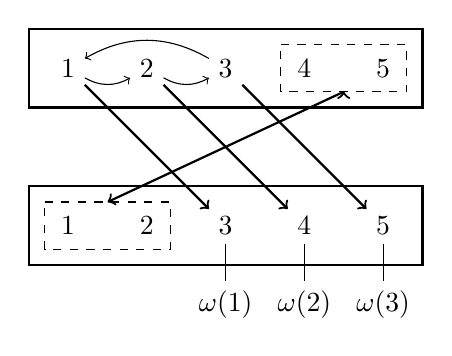
\begin{tikzpicture}
	\node (1) at (1,1) {$1$};
	\node (2) at (2,1) {$2$};
	\node (3) at (3,1) {$3$};
	\node (4) at (4,1) {$4$};
	\node (5) at (5,1) {$5$};
	
	\node (1p) at (1,-1) {$1$};
	\node (2p) at (2,-1) {$2$};
	\node (3p) at (3,-1) {$3$};
	\node (4p) at (4,-1) {$4$};
	\node (5p) at (5,-1) {$5$};
	
	\node (w1) at (3,-2) {$\omega(1)$};
	\node (w2) at (4,-2) {$\omega(2)$};
	\node (w3) at (5,-2) {$\omega(3)$};
	
	% flechas de alpha
	\draw[->] 	(1) edge[bend right] (2)
	(2) edge[bend right] (3)
	(3) edge[bend right] (1);
	
	% flechas de omega
	\draw[->,thick] (1) edge (3p)
	(2) edge (4p)
	(3) edge (5p)
	(4.5,0.7) edge (1.5,-0.7);
	
	\draw[=] 	(3p) -- (w1)
	(4p) -- (w2)
	(5p) -- (w3);
	
	\draw[thick] (0.5,1.5) -- (5.5,1.5) -- (5.5,0.5) -- (0.5,0.5) -- cycle;
	
	\begin{scope}[shift={(0,-2)}]
	\draw[thick] (0.5,1.5) -- (5.5,1.5) -- (5.5,0.5) -- (0.5,0.5) -- cycle;
	\end{scope}
	
	% cuadrao del 45		
	\draw[dashed] (3.7,1.3) -- (5.3,1.3) -- (5.3,0.7) -- (3.7,0.7) -- cycle;
	
	
	% cuadrao del 12
	\begin{scope}[shift={(-3,-2)}]
	\draw[dashed] (3.7,1.3) -- (5.3,1.3) -- (5.3,0.7) -- (3.7,0.7) -- cycle;
	\end{scope}
	
	\end{tikzpicture}
\end{wrapfigure}

¿Por qué es interesante esto? Porque los elementos de $cl(\alpha)$ son todas las permutaciones del mismo tipo que $\alpha$. Lo vemos con un ejemplo.



\begin{ej}
	% TODO entender esto
	Consideramos $\alpha \in S_5,\ \alpha = (123)$. Los elementos de la clase de equivalencia son de la forma $cl(\alpha) = \{\omega (123) \inv{\omega} \mid \omega \in S_5\}$. Es decir que, por ejemplo:
	\begin{align*}
		cl((123)(45)) &= \{(i_1\ i_2\ i_3)(i_4\ i_5) \mid \text{totalidad de elementos de tipo } (3,2)\}\\
		cl((12)) &= \{\text{elementos de clase } (2,1,1,1)\}
	\end{align*}
	
	
	Observemos que $\omega (123) \inv{\omega} = (\omega(1)\ \omega(2)\ \omega(3))$. Con $\omega = (12345)$ tenemos
	
	\begin{align*}
		\omega(123)\inv{\omega}(\omega(1)) = \omega(123)\inv{\omega}(3) = \omega(123)(\omega(1)) = \omega(2)\\
		\omega(123)\inv{\omega}(\omega(2)) = \omega(123)\inv{\omega}(2) = \omega(123)(\omega(2)) = \omega(3) \\
		\omega(123)(54)\inv{\omega} = (234)(15)
	\end{align*}
\end{ej}

\begin{ej}¿Cuántos elementos hay en la clase de equivalencia del elemento $(123) \in S_3$?
	
\begin{itemize}
	\item En $S_3$ los posibles tipos son $(3),\ (2,1),\ (1,1,1)$. El elemento $(123)$ que es de tipo $3$. 
	\item Por lo visto anteriormente sabemos que $cl((123)) = \{\text{totalidad elementos de tipo 3 en } S_3\}$. Por tanto, la pregunta en los grupos de permutaciones es ¿cuántos 3-ciclos hay en $S_3$?
	\item Recordemos que $|cl((123))| = [S_3: C((123))]$, luego solo necesitamos saber cuántos elementos hay en $C((123))$.
	\begin{itemize}
		\item Por el teorema de Lagrange (\autoref{thm:lagrange}) sabemos que los posibles órdenes del subgrupo $C((123))$ son $1,2,3,6$ (los divisores de $|S_3| = 6$).
		\item Sabemos que siempre $(123) \in C((123))$. Además $C((123))$ es un grupo, luego por clausura es necesario que $\gen{(123)} \subset S_3$. Esto nos dice que $|C((123))| \geq 3$.
		\item ¿Puede haber algún elemento más? No, porque $C((123))$ es un subgrupo propio. Esto quiere decir que tiene menos elementos que $S_3$ luego $|C((123)) < 6$.
		\item Entonces, $C((123))$ solo puede tener 3 elementos (y por tanto $C((123)) = \gen{(123)}$).
	\end{itemize}
	\item Concluímos que $|cl((123))| = [S_3:C((123))] = \frac{6}{3} = 2$. De hecho, los elementos son $cl(123) = \{(123), (132)\}$.
\end{itemize}
\end{ej}

\subsection{Estudio de un caso: descomposición detallada del grupo $S_4$}
\label{sec:descomposicons4}

A lo largo de los siguientes ejemplos veremos cómo se descompone $S_4$ en clases disjuntas de acuerdo a los tipos de sus permutaciones.

\begin{ej}
	Consideramos el grupo $S_4$. Queremos ver cómo se descompone $S_4$ en clases de equivalencia según los tipos de sus permutaciones.
	
	\begin{itemize}
		\item Los posibles tipos en $S_3$ son $4, 3+1, 2+2, 2+1+1, 1+1+1+1$. Recordemos que por la demostración del Teorema de Cauchy tenemos que
		\begin{align*}
			S_4 = cl((1234)) \cup cl((123)) \cup cl((12)(34)) \cup cl((12)) \cup cl(Id)
		\end{align*}
		Aquí, hemos tomado un representante de cada clase para escribirla más cómodamente. Lo que dice la ecuación de arriba es que $S_4$ está formado por todas las permutaciones de cada posible tipo que se puede dar en $S_4$.
		\item Nos preguntamos, por ejemplo, ¿cuántos elementos hay en $C((1234))$? Para averiguarlo utilizaremos que $[S_4:cl((1234))] = |C((1234))|$. El problema se reduce a averiguar $|cl((1234))|$ puesto que ya sabemos que $|S_4| = 4!$.
		\begin{itemize}
			\item En $cl((1234))$ están todos los 4-ciclos. ¿Cuántos hay? Tenemos que ver de cuántas maneras distintas podemos escribir 4 números $(i_1\ i_2\ i_3\ i_4)$ de manera que todas representen 4-ciclos diferentes.
			\item Como una \textit{rotación} de los números de un ciclo no cambia la permutación que describe (esto es, $(1234) = (2341)$) lo que buscamos es, fijado un número, de cuántas maneras podemos ordenar los demás. Es decir, ¿de cuántas maneras podemos ordenar 3 números distintos? Pues de $3! = 6$ maneras.
			\item Por último nos queda ver qué valores pueden tomar los 4 números que escribimos en el ciclo. Pues tenemos disponibles 4 números para elegir (del 1 al 4) y tenemos que coger 4, así que solo hay una manera, o lo que es lo mismo, hay $\binom{4}{4}$ maneras.
			\item Concluimos que en $cl((1234))$ hay $3! \binom{4}{4} = 6 \cdot 1 = 6$ 4-ciclos, y por tanto en $C((1234))$ hay $[S_4:cl((1234))] = \frac{24}{6} = 4$ elementos.
		\end{itemize}
		\item Ahora nos preguntamos lo mismo pero para los 3-ciclos, es decir, las permutaciones de tipo $3+1$. Procediendo de la misma manera obtenemos que el número de 3 ciclos es
		\begin{align*}
			|cl((123))| = \text{\# elementos a ordenar} \times \text{\# posibles valores } = (3-1)! \times \binom{4}{3} = 2! \cdot \frac{4!}{1!3!} = 8
		\end{align*}
		Con lo cual $|C((123))| = [S_4:cl((123))] = \frac{24}{8} = 3$
	\end{itemize}
\end{ej}

Podríamos seguir con el ejemplo anterior pero le daremos una vuelta más. En vez de pedir solo el orden del subgrupo $C((12)(34))$ como nos tocaría si siguieramos el orden lógico, pedimos los generados de ese subgrupo.

\begin{ej}
	Halla los generadores del subgrupo $C((12)(34)) < S_4$.
	
	\begin{itemize}
		\item Una buena manera de empezar, es preguntarse cuántos elementos hay en $C((12)(34))$ y para ello necesitamos saber cuántos elementos hay en $cl((12)(34))$. Esta vez es un poco más complicado.
		\begin{itemize}
			\item El número de posibles primeras parejas (primeros 2-ciclos) que podemos poner para obtener un elemento de tipo $2+2$ es $1! \times \binom{4}{2} = 6$.
			\item Observemos que al elegir la primera pareja queda determinada la segunda (solo hay 4 elementos para elegir).
			\item Observemos también que al ser ciclos disjuntos, reordenaciones de estas dos parejas no dan permutaciones distintas. Dividimos entre 2.
			\item Queda que $|cl((12)(34))| = 3$
			\item Una manera alternativa de pensar este caso es decir: fijo el 1 como primer elemento de la primera pareja. Para elegir el segundo solo me quedan 3 elementos y la segunda pareja me queda determinada en cuanto lo haga. Así que hay 3 permutaciones de tipo $2+2$.
		\end{itemize}
		\item Finalmente tenemos que $C((12)(34)) = \frac{24}{3} = 8$. Ya sabíamos que $\gen{(12)(34)} \subset C((12)(34))$ pero $o((12)(34)) = 2$ luego con los elementos de $\gen{(12)(34)}$ no tenemos suficientes para llenar $C((12)(34))$.
		
		\item Probamos con otros elementos $\tau$ de $S_4$ a ver si verifican $\tau(12)(34)\inv{\tau} = (12)(34)$:
		\begin{align*}
			\tau_1 = (1234)\qquad &\tau_1(12)(34)\inv{\tau_1} = (1234)(12)(34)\inv{(1234)} = (34)(12) = (12)(34)\\
			\tau_2 = (12)\qquad &\tau_2 (12)(34)\inv{\tau_2} = (12)(12)(34)\inv{(12)} = (34)(12) = (12)(34)
		\end{align*}
		De las ecuaciones anteriores tenemos que $(1234) \in C((12)(34)) \land (12) \in C((12)(34))$. Además, por clausura, $\gen{(1234)} = \{(1234), (12)(34), (4321), Id\} \subset C((12)(34)) \land \gen{(12)} = \{(12), Id\} \subset C((12)(34))$.
		\item Como $|\gen{(1234)}\cap \gen{(12)}| = 1$ tenemos, por el \autoref{thm:cardinalidadproductolibre}, que $|\gen{(1234)}\gen{(12)}| = |\gen{(1234), (12)}| = 4 \cdot 2 = 8 = |C((12)(34))| \implies C((12)(34)) = \gen{(1234), (12)}$ 
	\end{itemize}
\end{ej}

\begin{ej}
	Halla los generadores del subgrupo centralizador del elemento $(12)$ en $S_4$
	
	\begin{itemize}
		\item $|C((12)) = [S_4:cl((12))]$. Obtenemos $cl((12))$ de la manera habitual: número de 2-ciclos = $(2-1)! \times \binom{4}{2} = 6$. Por tanto $|C((12)) = 24/6 = 4$.
		
		\item Sabemos que $\gen{(12)} \subset C((12))$ luego necesitamos otros dos elementos para rellenar $C((12))$.
		\item Pues vamos a probar a ver qué pasa con $(34)$:
		\begin{align*}
			(34)(12)\inv{(34)} = (12)(34)\inv{(34)} = (12) \implies (34) \in C((12)) \implies \gen{(34)} \subset C((12))
		\end{align*}
		\item Como en el ejemplo anterior aplicamos el \autoref{thm:cardinalidadproductolibre} y obtenemos que $|\gen{(12)}\gen{34}| = |\gen{(12), (34)}| = \frac{|\gen{(12)}||\gen{(34)}|}{|\gen{(12)} \cap \gen{(34)}|} = \frac{2\cdot2}{1} \implies C((12)) = \gen{(12), (34)}$
	\end{itemize}
\end{ej}

Recapitulando comprobamos que $S_4$ se descompone en
\begin{itemize}
	\item 6 4-ciclos (tipo $4$),
	\item 8 3-ciclos (tipo $3+1$),
	\item 3 2-ciclos $+$ 2-ciclos (tipo $2+2$),
	\item 6 2-ciclos (tipo $2+1+1$), y
	\item 1 identidad o 1-ciclo (tipo $1+1+1+1$).
\end{itemize}
En total suman 24 elementos.

\subsection{Conjugación}

\begin{thm}[Lema del conjugado]
	
\end{thm}

\section{Clases de equivalencia de subgrupos en $S_n$}

Ahora haremos lo mismo que hemos hecho para permutaciones pero con subgrupos. Recordemos que el normalizador es lo mismo que el centralizador pero aplicado a subgrupos: el normalizador de un subgrupo son las permutaciones que mandan a un subgrupo en sí mismo mientras que en el caso del centralizador eran los elementos que mandan un elemento en sí mismo.

Conviene recordad la definición \ref{dfn:normalizador} y la \autoref{pro:centralizadorsubgruponormalizador}.

\begin{ej}
	Entender y copiar ejemplo pág 100 santorum
\end{ej}

\section{[Sub]grupos alternados}
\label{sec:gruposalternados}

Recordemos que existía un homomorfismo de grupos $S_n  \to (\{-1, 1\}, \cdot)$ y que defiamos la paridad de una permutación $\sigma \in S_n$ como par si $\sigma \mapsto 1$ y como impar si $\sigma \mapsto -1$. Esto tenía sentido porque una permutación par se descomponía siempre en un número par de transposiciones y ocurría lo mismo con las permutaciones impares.

Pues resulta que nos interesa mucho el conjunto formado por las trasposiciones de orden par. Esto conjunto es en realidad un subgrupo (recordar que la paridad se mantiene si operamos con trasposicones de la misma paridad) y además veremos que es un subgrupo normal de $S_n$.

\begin{dfn}[Grupo alternado]
	Sea $\varphi: S_n \to ({-1, 1}, \cdot)$ el homomorfismo de grupos definido arriba. Definimos el grupo alternado o alternante $A_n$ como
	\begin{align*}
	A_n = \ker \varphi = \{\sigma \in S_n \mid \sigma \text{ es par}\}
	\end{align*}
\end{dfn}

Recogemos los resultados que hemos dejado caer antes de la definición:

\begin{pro}
	$A_n \normsub S_n$ y además $[S_n : A_n] = 2$
\end{pro}

\begin{cor}
	Todo grupo $S_n$ tiene un subgrupo normal de orden $2$.
\end{cor}

Hay dos resultados más que aún no entiendo para qué sirven:

\begin{pro}
	\begin{align*}
		S_n / A_n \isom (\{-1, 1\}, \cdot)
	\end{align*}
\end{pro}

\begin{pro}
	Todo subgrupo normal de $S_n$ se puede expresar como unión de cajas.
\end{pro}

Pasado esto seguimos con nuestras vidas. Veamos ejemplos.

\begin{ej}
	Consideramos $|S_5| = 5! = 120$. Haciendo lo mismo que hicimos para $S_4$ en la sección \ref{sec:descomposicons4} obtenemos lo siguiente:
	\begin{table}[h]
		\centering
		{\renewcommand{\arraystretch}{1.3}
		\begin{tabular}{|l|l|l|}
			\hline
			\textbf{tipo $5$}       & $|cl((12345))| = 4! \binom{5}{5} = 24$   & $C((12345)) = \gen{(12345)} \isom \Z/5\Z$       \\ \hline
			\textbf{tipo $4+1$}     & $|cl((1234))| = 3! \binom{5}{4} = 30$    & $C((1234)) = \gen{(1234)} \isom \Z/4\Z$         \\ \hline
			\textbf{tipo $3+2$}     & $|cl((123)(45))| = 2! \binom{5}{2} = 20$ & $C((123)(45)) = \gen{(123),(45)} \isom \Z/6\Z$  \\ \hline
			\textbf{tipo $3+1+1$}   & $|cl((123))| = 2! \binom{5}{2} = 20$     & $C((123)) = \gen{(123),(45)} \isom \Z/6\Z$      \\ \hline
			\textbf{tipo $2+2+1$}   & $|cl((12)(34))| = 15$                    & $C((12)(34)) = \gen{(1234),(13)} \isom D_4$     \\ \hline
			\textbf{tipo $2+1+1+1$} & $|cl((12))| = 1! \binom{5}{2} = 10$      & $C((12)) = \gen{(12345)} \isom H \times \Z/2\Z$ \\ \hline
			\textbf{tipo $1+1+1+1$} & $|cl((1) = Id)| = 1$                     & $C(Id) = S_5$                                   \\ \hline
		\end{tabular}}
		\caption{Descomposición de $S_5$ en clases. Nota: aquí $H \isom S_3$ o bien $H = \{\sigma \in S_5 \mid \sigma(1) = 1 \land \sigma(2) = 2\}$}
		\label{fig:descomposicons5}
	\end{table}

	¿Cuáles son los tipos que estarían en $A_5$? Pues aquellos que se puedan descomponer en un número par de trasposiciones. A saber: tipo $5$, tipo $3+1+1$, tipo $2+2+1$, tipo $2+1+1+1$. Por tanto en $|A_5| = 24 + 20 + 15 + 1 = 60 \implies [S_5:A_5] = 2 \implies A_5 \normsub S_5$.
\end{ej}

\begin{obs}
	En $S_n$ siembre hay un subgrupo isomorfo a $D_n$.
	
	Lo construimos buscando un elemento $B \in S_n$ de orden $n$ (pista, el elemento $(123\dots n)$ siempre vale) y otro elemento $A \in S_n$ de orden dos tal que $BA = A\inv{B}$. Con esto llegamos a la presentación de $D_n$. Ver \autoref{ej:diedricosordengenerico} para más detalles sobre esta presentación.
\end{obs}

\section{Grupos simples}

\begin{dfn}[Grupo simple]
	\label{dfn:simple}
	Sea $G$ un grupo, decimos que $G$ es un grupo simple si los únicos grupos normales son $G$ y el grupo neutro $\{e\}.$
\end{dfn}

A continuación demostraremos que el grupo alternante $A_n$, es simple para $n\geq 5$. La demostración de este resultado requiere distintas proposiciones.
\begin{pro}
	Sea $G$ un grupo. Si $G$ es finito y abeliano $\implies\ G$ es simple.
\end{pro}
%TODO: demostracion de la proposición.
\begin{pro}
	Sea $A_n$ un grupo alternante, $A_n$ es generado por 3-ciclos para $n\geq 3$.
\end{pro}
\begin{proof}
	Sea $\sigma \in A_n$, entonces $\sigma = (i_1^1\ i_2^1)(i_1^2\ i_2^2)\ldots(i_1^{2n}\ i_2^{2n})$ una composición de un número par de composiciones. Vamos a ver que para cualquier par de transposiciones $(i\ j)(k\ l)$ podemos expresarla como un $3-ciclo$.
	\begin{align*}
	(i\ j)(k\ l) &= (i\ k\ j)(i\ k\ l)\ &si\ los\ elementos\ son\ diferentes.\\
	(i\ j)(i\ l) &= (i\ l\ j)\ &si\ tienen\ un\ elemento\ en\ comun.
	\end{align*}
	Por tanto, como $\forall \sigma \in A_n$ puede ser expresado como un $3-ciclo$ o una composición de estos, $A_n$ está generado por los ciclos de longitud 3.
\end{proof}
\begin{pro}
	\label{pro:alternante3ciclos}
	Sea $A_n$ el grupo alternante de un conjunto de $n$ elementos, $A_n$ es generado por 3-ciclos de la forma $(s\ t\ i)$ con $s,t\in \{1\ldots n\}$ fijos e $i\in\{1\ldots n\}\setminus\{s,t\}$
\end{pro}
\begin{proof}
	Cada 3-ciclo es el producto de 3-ciclos del tipo $(s\ t\ i)$ con $s,t$ fijos e $i$ variable, pues:
	\begin{align*}
	(s\ a\ t) &= (s\ t\ a)^2\\
	(s\ a\ b) &= (s\ t\ b)(s\ t\ a)^2\\
	(t\ a\ b) &= (s\ t\ b)^2(s\ t\ a)\\
	(a\ b\ c) &= (s\ t\ a)^2(s\ t\ c)(s\ t\ b)^2(s\ t\ a)
	\end{align*}
	Entonces, como $A_n$ está generado por 3-ciclos, $A_n$ está generado por ciclos de la forma $(s\ t\ i)$
\end{proof}
\begin{thm}[Igualdad entre subgrupos y grupos alternantes]
	\label{thm:subequalsalternate}
	Si un subgrupo normal $H$ de $A_n$ contiene un 3-ciclo $\implies H = A_n$
\end{thm}
\begin{proof}
	Supongamos que $H$ es no trivial y contiene un 3-ciclo de la forma $(s\ t\ a)$. Usando la normalidad de $H$ vemos que:
	\[
	[(s\ t)(a\ i)](s\ t\ a)^2[(s\ t)(a\ k)]^{-1} = (s\ t\ i)
	\]
	está en $H$. Luego, $H$ debe contener todos los ciclos $(s\ t\ i)$ para $1 \geq i \geq n$. Por la \autoref{pro:alternante3ciclos}, estos 3-ciclos generan $A_n$; luego $H = A_n$.
\end{proof}
\begin{pro}
	\label{pro:3cicloinsubgralter}
	Para $n\geq 5$, todo $H \normsub A_n$ contiene un 3-ciclo.
\end{pro}
\begin{proof}
	Sea $e \not \eq \sigma \in H$, existen varias posibles estructuras de ciclos para $\sigma$.
	\begin{itemize}
		\item $\sigma$ es un 3-ciclo.
		\item $\sigma$ es el producto de ciclos disjuntos, $\sigma = \tau(a_1\ a_2 \cdots a_r)\in H$, con $r\geq 3$.
		\item $\sigma$ es el producto de ciclos disjuntos, $\sigma = \tau(a_1\ a_2\ a_3)(a_4\ a_5\ a_6)$.
		\item $\sigma = \tau(a_1\ a_2\ a_3)$, donde $\tau$ es el producto de 2-ciclos disjuntos.
		\item $\sigma = \tau(a_1\ a_2)(a_3\ a_4)$, donde $\tau$ es el producto de un número par de 2-ciclos disjuntos.
	\end{itemize}
	La demostración sigue con el desarrollo de cada uno de los casos, utilizando la normalidad de $H$ para ver que en todos los casos se llega a que $H$ contiene un 3-ciclo.
\end{proof}
\begin{thm}[Simplicidad del grupo alternante]
	Sea $(A_n, \circ)$ el grupo alternante de un conjunto de $n$ elementos. $A_n$ es simple $\forall n \geq 5$.
\end{thm}
\begin{proof}
	Sea $H$ un subgrupo normal no trivial de $A_n$, por la  \autoref{pro:3cicloinsubgralter}, $H$ contiene un 3-ciclo. Por el  \autoref{thm:subequalsalternate}, $H = A_n$; por tanto, $A_n$ no contienen ningún subgrupo normal que sea propio y no trivial para $n\geq 5$.
\end{proof}

